\documentclass[11pt,letterpaper]{article}

\usepackage[margin=0.78in,headheight=24pt]{geometry}
\usepackage[T1]{fontenc}
\usepackage[utf8]{inputenc}
\usepackage{array,booktabs,tabularx,longtable}
\usepackage{amsmath,amssymb}
\usepackage{enumitem}
\usepackage{fancyhdr}
\usepackage{graphicx}
\usepackage{hyperref}
\usepackage{listings}
\usepackage{xcolor}
\usepackage{titlesec}
\usepackage{parskip}
\usepackage{tikz}
\usepackage[expansion=false]{microtype}
\usetikzlibrary{arrows.meta,positioning,fit,shapes.geometric,backgrounds}

\definecolor{leafcyan}{RGB}{0,137,140}
\definecolor{leafgreen}{RGB}{48,145,91}
\definecolor{leafamber}{RGB}{205,132,35}
\definecolor{leafred}{RGB}{180,67,67}
\definecolor{leafink}{RGB}{34,41,47}
\definecolor{leafmuted}{RGB}{91,103,113}
\definecolor{leafpanel}{RGB}{244,248,248}
\definecolor{leafline}{RGB}{199,216,216}
\definecolor{leafcode}{RGB}{239,244,244}
\definecolor{leafnavy}{RGB}{34,63,87}

\hypersetup{
  colorlinks=true,
  linkcolor=leafcyan,
  urlcolor=leafcyan,
  citecolor=leafcyan,
  pdftitle={LeafOS Small-Scale MoE and Unified Hardware Orchestration},
  pdfsubject={Proposed architecture for local micro-MoE routing and hardware utilization},
  pdfauthor={LeafOS}
}

\pagestyle{fancy}
\fancyhf{}
\lhead{\textcolor{leafmuted}{LeafOS Architecture}}
\rhead{\textcolor{leafmuted}{Micro-MoE Hardware Orchestration}}
\cfoot{\textcolor{leafmuted}{\thepage}}
\renewcommand{\headrulewidth}{0.3pt}
\renewcommand{\headrule}{\hbox to\headwidth{\color{leafline}\leaders\hrule height \headrulewidth\hfill}}

\titleformat{\section}{\Large\bfseries\color{leafcyan}}{}{0pt}{}[\titlerule]
\titleformat{\subsection}{\large\bfseries\color{leafink}}{}{0pt}{}
\titleformat{\subsubsection}{\normalsize\bfseries\color{leafnavy}}{}{0pt}{}
\setlist{leftmargin=1.4em,itemsep=2pt,topsep=4pt}
\setlength{\emergencystretch}{3em}

\lstdefinestyle{leaf}{
  basicstyle=\ttfamily\footnotesize,
  breaklines=true,
  backgroundcolor=\color{leafcode},
  frame=single,
  rulecolor=\color{leafline},
  xleftmargin=8pt,
  xrightmargin=8pt,
  aboveskip=7pt,
  belowskip=7pt,
  showstringspaces=false,
  columns=fullflexible,
  keepspaces=true
}
\lstset{style=leaf}

\newcolumntype{L}[1]{>{\raggedright\arraybackslash}p{#1}}
\newcolumntype{Y}{>{\raggedright\arraybackslash}X}
\newcommand{\code}[1]{\texttt{#1}}
\newcommand{\status}[2]{%
  \fcolorbox{leafline}{#1}{\strut\hspace{5pt}#2\hspace{5pt}}}
\newcommand{\callout}[2]{%
  \begin{center}
  \fcolorbox{leafline}{leafpanel}{%
    \begin{minipage}{0.94\linewidth}
      \textbf{\textcolor{leafcyan}{#1}}\quad #2
    \end{minipage}}
  \end{center}}
\newcommand{\decision}[1]{\callout{Decision}{#1}}
\newcommand{\invariant}[1]{\callout{Invariant}{#1}}
\newcommand{\risk}[1]{\textcolor{leafred}{\textbf{#1}}}

\begin{document}
\hypersetup{pageanchor=false}

\begin{titlepage}
\thispagestyle{empty}
  \centering
  \vspace*{1.0cm}
  {\color{leafcyan}\rule{\linewidth}{2pt}}\\[0.55cm]
  {\Huge\bfseries\color{leafink} LeafOS Small-Scale MoE}\\[0.18cm]
  {\Huge\bfseries\color{leafink} and Unified Hardware Orchestration}\\[0.4cm]
  {\Large\color{leafmuted} A CPU-authoritative, GPU-leased micro-MoE execution plane}\\[0.55cm]
  {\color{leafcyan}\rule{\linewidth}{1pt}}\\[0.9cm]

  \begin{tabular}{rl}
    \textbf{Status:} & Proposed architecture \\
    \textbf{Design version:} & 0.6.0-design.2 \\
    \textbf{Prepared:} & 2026-07-26 \\
    \textbf{Primary input:} & \code{LeafOS\_Unified\_Hardware\_Orchestrator.ipynb} \\
    \textbf{Target host:} & Intel Core i9-13900K, RTX 4070 12 GB, 48 GB RAM \\
  \end{tabular}

  \vfill

  \begin{center}
    \status{leafgreen!16}{CPU is authority}
    \quad
    \status{leafcyan!13}{one GPU lease}
    \quad
    \status{leafamber!16}{adaptive top-1 to top-2}
  \end{center}

  \vspace{0.7cm}
  \fcolorbox{leafline}{leafpanel}{%
    \begin{minipage}{0.88\linewidth}
      \small
      This document locks in a hybrid mixture-of-experts architecture. LeafOS
      performs auditable routing between specialized model and tool workers at
      the work-object boundary. A routed model may itself use token-level sparse
      experts. The design seeks useful saturation of CPU, GPU, memory, and
      storage while preserving thermal, safety, and interactive headroom.
    \end{minipage}}

  \vfill
  {\small\color{leafmuted}
  Local-first. File-backed. Audit-first. No model directly mutates authoritative state.}
\end{titlepage}

\hypersetup{pageanchor=true}
\pagenumbering{roman}
\tableofcontents
\newpage
\pagenumbering{arabic}

\section{Executive decision}

\decision{Use a two-tier micro-MoE. LeafOS routes each typed work object to one
specialized expert by default and activates a second expert only when risk,
uncertainty, disagreement, or failed evidence justifies the cost. The selected
expert may be a dense model or an internally sparse MoE.}

The target system is not a new neural network training framework. It is a local
execution architecture that combines:

\begin{enumerate}
  \item a deterministic CPU control plane;
  \item a single exclusive GPU lease for the current hot model;
  \item CPU-side model, tool, verification, and data workers;
  \item RAM-backed warm state and SSD-backed cold state;
  \item evidence-gated promotion of model proposals into durable artifacts; and
  \item profile-driven utilization that can approach saturation only when useful
        queued work, telemetry, and policy allow it.
\end{enumerate}

The normal path is top-1 routing. Top-2 is a targeted escalation, not permanent
fan-out. This prevents a nominal ``swarm'' from doubling latency and energy for
routine tasks. Model changes, accelerator allocations, and corrective retries
remain explicit ledger events.

\subsection{Locked architectural choices}

\begin{tabularx}{\linewidth}{@{}L{0.25\linewidth}Y Y@{}}
\toprule
\textbf{Concern} & \textbf{Decision} & \textbf{Reason} \\
\midrule
MoE boundary &
Hybrid: LeafOS work-object routing plus optional internal sparse MoE &
Preserves role specialization and auditability while exploiting sparse model
inference where available. \\
GPU ownership &
One GPU-backed hot expert at a time on the target host &
The installed model set does not safely permit two medium models to remain
fully resident in 12 GB VRAM with KV and runtime headroom. \\
Routing width &
Top-1 normally; top-2 after explicit escalation predicates &
Makes quality spending proportional to risk and uncertainty. \\
Control authority &
CPU parser, policy, validation, and durable writer &
Models produce proposals; they do not directly change task, graph, filesystem,
or node truth. \\
Utilization objective &
Useful throughput under a profile-specific latency and safety envelope &
Blind utilization can create model-load thrash, thermal throttling, and worse
interactive latency. \\
State authority &
Hash-chained JSONL journal and atomic checkpoints; SQLite may index them &
Matches LeafOS file-backed doctrine while allowing efficient local queries. \\
\bottomrule
\end{tabularx}

\section{Status, scope, and authority}

This is a proposed architecture document. It defines contracts and acceptance
gates; it does not claim that the current checkout implements them. The current
checkout is missing delegated taskpack entrypoints and several canonical
taskpack documents. Therefore:

\begin{itemize}
  \item existing run artifacts and accepted tests outrank design intention;
  \item this design must be promoted through the release evidence process;
  \item paths under the missing taskpack tree are proposed integration targets;
  \item illustrative notebook capacities are not performance claims; and
  \item provider flags are versioned capabilities, not permanent API promises.
\end{itemize}

\subsection{Primary inputs}

\begin{tabularx}{\linewidth}{@{}L{0.32\linewidth}Y@{}}
\toprule
\textbf{Input} & \textbf{Contribution} \\
\midrule
\path{LeafOS_Unified_Hardware_Orchestrator.ipynb} &
Compatible-claim scheduling, priority tiers, LIFO locality, correction lineage,
tiered placement, evidence gates, data tracks, operating modes, and TUI gates. \\
\code{docs/releases/STAGE.md} &
CPU authority, GPU/NPU worker boundary, file-backed state, adaptive resource
headroom, durable journals, and promotion rules. \\
\path{ProjectLeaf/leaf_model_installer/} &
Installed model inventory, runtime role policy, acquisition safety, GGUF
metadata, and the target-host preflight record. \\
\code{floweros\_hardware\_monitor/} &
Available CPU, RAM, storage, network, NVIDIA, temperature, fan, and power
telemetry plus explicit estimated-sensor behavior. \\
\code{llama.cpp} documentation and local build &
CPU/GPU hybrid inference, continuous batching, model router mode, metrics,
dynamic load/unload, sleep, and MoE CPU placement controls. \\
\bottomrule
\end{tabularx}

\section{Goals and non-goals}

\subsection{Goals}

\begin{itemize}
  \item Keep the strongest feasible expert hot for the current workload without
        allowing model residency to become hidden global state.
  \item Use idle CPU, GPU, memory, and storage capacity for useful, preemptible
        work without delaying critical interaction.
  \item Route work by capability, risk, measured quality, residency, transfer
        cost, and current pressure.
  \item Make every routing, placement, model-load, validation, repair, and
        promotion decision reconstructable from durable records.
  \item Bound retries, correction depth, queue starvation, memory pressure, and
        accelerator contention.
  \item Support one host today and preserve a logical-worker boundary suitable
        for later multi-node placement.
\end{itemize}

\subsection{Non-goals}

\begin{itemize}
  \item Training a token-level MoE foundation model.
  \item Pretending SSD-backed capacity implies useful interactive throughput.
  \item Treating multiple devices as unified VRAM without backend evidence.
  \item Keeping every installed model resident.
  \item Using model consensus as a substitute for deterministic tests.
  \item Allowing overnight jobs to modify the live source tree without a later
        approval and integration gate.
  \item Maximizing utilization when no valuable work is ready.
\end{itemize}

\section{Evidence baseline}

\subsection{Target host}

The design is calibrated first for the current LeafOS host, not for the
notebook's illustrative 24 GB and 48 GB dual-GPU workers.

\begin{tabularx}{\linewidth}{@{}L{0.25\linewidth}L{0.27\linewidth}Y@{}}
\toprule
\textbf{Resource} & \textbf{Observed} & \textbf{Architectural consequence} \\
\midrule
CPU &
Intel Core i9-13900K, 24 cores, 32 logical processors &
Enough concurrency for control, validation, build/test, retrieval, and a
bounded CPU inference lane. Topology must be discovered rather than hard-coded. \\
GPU &
NVIDIA GeForce RTX 4070, 12,282 MiB VRAM, 200 W reported limit &
One exclusive hot-model lease. NVIDIA telemetry is authoritative over WMI
adapter-memory fields. \\
RAM &
48 GiB Kingston module, configured at 4800 MT/s &
Capacity for memory-mapped cold weights and CPU workers, but memory bandwidth
must be measured before promising CPU-MoE throughput. \\
Storage &
2 TB SHPP41 NVMe SSD &
Cold model and artifact tier. Placement scores must account for transfer
amplification and random expert access. \\
Operating system &
Windows 11, build 26200 &
Power, process priority, affinity, and sensor behavior must remain
platform-adapter concerns. \\
\bottomrule
\end{tabularx}

\subsection{Installed model assets}

\begin{tabularx}{\linewidth}{@{}L{0.25\linewidth}L{0.12\linewidth}L{0.18\linewidth}Y@{}}
\toprule
\textbf{Artifact} & \textbf{Size} & \textbf{Architecture} & \textbf{Proposed role} \\
\midrule
Gemma4 Coder Q4\_K\_M &
6.87 GiB & dense, 48 blocks & Primary coding expert. \\
Gemma4 Opus Assistant Q4\_K\_M &
6.87 GiB & dense, 48 blocks & Main/architect expert and planning fallback. \\
Qwopus 9B Coder MTP Q4\_K\_M &
5.38 GiB & dense, 33 blocks & Optional fast coder, draft, or repair candidate after calibration. \\
Qwen3.5 reasoning MXFP4\_MOE &
8.23 GiB & sparse, 40 blocks, 93 experts, 8 used & Selective deep reasoning and critic expert. \\
Qwen3.5 vision projector &
0.57 GiB & vision encoder & On-demand visual specialist; not permanently resident. \\
\bottomrule
\end{tabularx}

\risk{Identity discrepancy.} The reasoning filename and catalog describe
``14B-A3B'', while embedded GGUF metadata identifies
``Qwen3.5 35B A3B'' with 93 experts and 8 experts used per token. LeafOS must
derive runtime identity from a content hash plus inspected metadata, compare it
with the catalog, and refuse default promotion while material fields disagree.
An explicit experimental override may permit measured evaluation.

\subsection{Notebook verification}

The notebook contains no saved outputs, so its code cells were executed as one
in-memory asynchronous program. The following prototype properties passed:

\begin{itemize}
  \item five scheduled tasks completed;
  \item the critic ran only on a compatible worker;
  \item declared VRAM bounds held;
  \item the correction cascade remained below its configured limit;
  \item evidence-backed quality measurements produced an accepted decision;
  \item evaluation holdout data remained excluded from training; and
  \item seven-page TUI navigation wrapped and reversed correctly.
\end{itemize}

These are semantic checks. They do not measure inference speed, SSD streaming,
KV growth, thermal stability, or provider cancellation.

\subsection{Final design audit: prototype corrections}

The notebook is a useful executable sketch, but its production boundary contains
four correctness hazards that this architecture intentionally does not preserve:

\begin{tabularx}{\linewidth}{@{}L{0.27\linewidth}Y@{}}
\toprule
\textbf{Prototype shortcut} & \textbf{Production correction} \\
\midrule
RAM and SSD capacities are added &
Treat VRAM, resident RAM, and durable storage as separate constraints. A
memory-mapped artifact still occupies SSD while some pages are resident in RAM;
the same bytes cannot be counted as interchangeable free capacity. \\
Heap storage is scanned by array order &
Claim from a stable scheduling-ordered index. A binary heap guarantees only its
root is minimal; iterating its backing array is not a total priority order. \\
Ledger sequence is computed before locking &
One durable writer allocates the sequence and previous hash inside the append
critical section, then flushes the canonical record before publishing it. \\
Provider completion is treated as task completion &
Provider return produces a proposal. Verification, acceptance, and durable
completion remain separate states. \\
\bottomrule
\end{tabularx}

The notebook's two-GPU examples also remain illustrative. This document targets
the observed single-GPU host and treats any future multi-device placement as one
backend-owned logical allocation.

\section{Architectural invariants}

\invariant{A model response is a proposal. Only CPU-side schema, scope, policy,
and evidence gates can accept it as an authoritative artifact.}

\begin{enumerate}
  \item \textbf{Typed work first.} Human or model text is parsed into a versioned
        work envelope before scheduling.
  \item \textbf{Eligibility before scoring.} An expert that violates capability,
        scope, memory, safety, or availability constraints is never ranked.
  \item \textbf{One accelerator owner.} Exactly one GPU lease may be active on
        the target single-GPU host. The lease is exclusive among LeafOS
        allocations; non-LeafOS VRAM use is observed and deducted.
  \item \textbf{No false completion.} Queued, claimed, started, proposed,
        validated, accepted, failed, and cancelled are distinct states.
  \item \textbf{Durable before dependent side effects.} The journal transition
        is flushed before a subsequent mutation depends on it.
  \item \textbf{Bounded correction.} Repair depth, attempts, wall time, tokens,
        and affected paths are explicit budgets.
  \item \textbf{Telemetry provenance.} Estimated temperature or fan values are
        labeled and cannot authorize a high-risk thermal decision.
  \item \textbf{Useful work only.} Background load is immediately preemptible
        and cannot block a critical model load.
  \item \textbf{No exactly-once fiction.} Crash recovery is at-least-once.
        Side effects are idempotent or reconciled before retry, and stale
        claim epochs cannot publish results.
  \item \textbf{Artifacts beat intention.} Accepted tests and run evidence
        outrank design prose when they disagree.
\end{enumerate}

\section{Reference architecture}

\begin{figure}[ht]
\centering
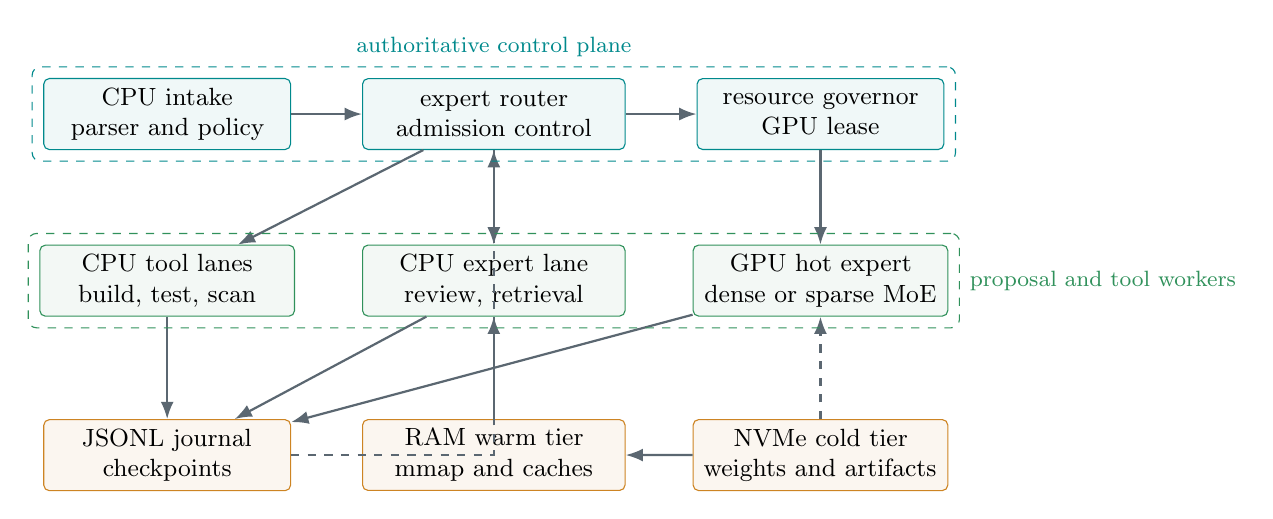
\begin{tikzpicture}[
  node distance=7mm and 9mm,
  box/.style={draw=leafline, rounded corners=2pt, fill=leafpanel,
              minimum height=9mm, align=center, font=\small},
  core/.style={box, draw=leafcyan, fill=leafcyan!6},
  worker/.style={box, draw=leafgreen, fill=leafgreen!6},
  store/.style={box, draw=leafamber, fill=leafamber!7},
  arrow/.style={-{Latex[length=2.2mm]}, thick, color=leafmuted}
]
  \node[core, text width=29mm] (intake) {CPU intake\\parser and policy};
  \node[core, text width=31mm, right=of intake] (router) {expert router\\admission control};
  \node[core, text width=29mm, right=of router] (lease) {resource governor\\GPU lease};

  \node[worker, text width=30mm, below=12mm of intake] (tools) {CPU tool lanes\\build, test, scan};
  \node[worker, text width=31mm, below=12mm of router] (cpu) {CPU expert lane\\review, retrieval};
  \node[worker, text width=30mm, below=12mm of lease] (gpu) {GPU hot expert\\dense or sparse MoE};

  \node[store, text width=29mm, below=13mm of tools] (journal) {JSONL journal\\checkpoints};
  \node[store, text width=31mm, below=13mm of cpu] (ram) {RAM warm tier\\mmap and caches};
  \node[store, text width=30mm, below=13mm of gpu] (ssd) {NVMe cold tier\\weights and artifacts};

  \draw[arrow] (intake) -- (router);
  \draw[arrow] (router) -- (lease);
  \draw[arrow] (router) -- (tools);
  \draw[arrow] (router) -- (cpu);
  \draw[arrow] (lease) -- (gpu);
  \draw[arrow] (tools) -- (journal);
  \draw[arrow] (cpu) -- (journal);
  \draw[arrow] (gpu) -- (journal);
  \draw[arrow] (ram) -- (cpu);
  \draw[arrow] (ssd) -- (ram);
  \draw[arrow, dashed] (ssd) -- (gpu);
  \draw[arrow, dashed] (journal) -| (router);

  \node[draw=leafcyan, dashed, rounded corners=3pt, fit=(intake)(router)(lease),
        inner sep=4pt, label={[font=\footnotesize\color{leafcyan}]above:authoritative control plane}] {};
  \node[draw=leafgreen, dashed, rounded corners=3pt, fit=(tools)(cpu)(gpu),
        inner sep=4pt, label={[font=\footnotesize\color{leafgreen}]right:proposal and tool workers}] {};
\end{tikzpicture}
\caption{Single-host LeafOS micro-MoE execution plane. Dashed storage-to-GPU
transfer is admitted only through the resource governor.}
\end{figure}

The control plane sees each provider allocation as a logical worker. It does
not split model tensors itself. CUDA, Vulkan, CPU offload, internal MoE expert
placement, and future multi-GPU groups remain inference-backend
responsibilities. LeafOS records and reasons over the resulting placement.

\section{Two-tier micro-MoE}

\subsection{Tier 1: LeafOS work-object experts}

Tier 1 is a system-level mixture of specialized workers. Its routing granularity
is a work object or graph node, not a token.

\begin{tabularx}{\linewidth}{@{}L{0.20\linewidth}L{0.24\linewidth}Y@{}}
\toprule
\textbf{Expert class} & \textbf{Default candidate} & \textbf{Authority and use} \\
\midrule
Architect/main &
Gemma4 assistant &
Plans, explains, decomposes, and proposes graph changes. Never writes graph
truth directly. \\
Coder &
Gemma4 coder &
Produces bounded patches or code artifacts within declared paths. \\
Deep critic &
Qwen sparse reasoning model &
Invoked for architectural risk, low confidence, broad dependency impact, or
failed integration evidence. \\
Fast repair/draft &
Qwopus coder candidate &
Optional low-latency repair or speculative lane after compatibility and quality
calibration. \\
Deterministic verifier &
Compiler, tests, linters, scanners &
Produces hard evidence. This is a tool worker, not an LLM vote. \\
Retrieval/embedding &
Small CPU or accelerator worker &
Builds compact evidence records when interactive work does not need the
resource. \\
Vision &
On-demand multimodal worker &
Inspects screenshots, plots, diagrams, OCR, and visual regression artifacts. \\
Overnight consolidator &
Strongest feasible reasoner on a frozen snapshot &
Produces proposals and work orders only; it cannot silently change the live
tree. \\
\bottomrule
\end{tabularx}

\subsection{Tier 2: internal sparse experts}

An eligible Tier 1 model may contain its own learned token router. LeafOS does
not override token routing. It may choose backend placement controls such as
keeping some MoE weights on CPU, but only through a measured placement profile.

The two routing levels have different evidence:

\begin{itemize}
  \item Tier 1 records expert eligibility, route score, selected endpoint,
        alternatives, escalation reason, and result disposition.
  \item Tier 2 records model identity, backend placement, tokens, latency,
        memory, and provider metrics. Per-token expert traces are optional
        diagnostics and are not required for control-plane correctness.
\end{itemize}

\subsection{Top-1 and top-2 policy}

\begin{tabularx}{\linewidth}{@{}L{0.25\linewidth}Y@{}}
\toprule
\textbf{Condition} & \textbf{Routing behavior} \\
\midrule
Routine, low-risk, known domain &
Top-1 expert; deterministic verification still applies. \\
Low router confidence &
Top-2 independent review or a stronger critic, subject to budget. \\
High-risk paths or security-sensitive work &
Top-1 generation plus mandatory critic and hard security gates. \\
Failed hard gate &
Structured repair packet routed to the best eligible repair expert. \\
Model disagreement &
Do not average prose. Compare claims against specification and tool evidence;
escalate unresolved differences to review. \\
Repeated failure or exhausted budget &
Quarantine or review-required. No immortal correction loop. \\
\bottomrule
\end{tabularx}

\paragraph{Single-GPU execution semantics.}
Top-2 describes two independent decisions, not two mandatory simultaneous GPU
residencies. Two GPU-backed experts execute sequentially under the same lease
manager, including any measured model-switch cost. Parallel top-2 is permitted
only when the allocations are resource-disjoint, such as a GPU proposal
overlapped with CPU tools or a bounded CPU critic. A projector and its base
model count as one composite placement bundle with one combined memory budget.

\subsection{Routing score}

Eligibility is a hard filter. For eligible expert \(e\) and work object \(w\),
the initial score is:

\[
R(e,w) =
\alpha C_{cap}
+ \beta Q_{hist}
+ \gamma H_{resident}
+ \delta S_{specialty}
- \epsilon L_{queue}
- \zeta T_{transfer}
- \eta L_{latency}
- \theta P_{pressure}
\]

where capability and policy violations are never represented as large
penalties; they make the expert ineligible. Weights are profile-specific and
versioned. Historical quality is scoped by task family and evidence, not a
single global reputation number.

Every score component is calibrated to \([0,1]\) before weighting; otherwise
latency in milliseconds could dominate a dimensionless quality term by accident.
\(Q_{hist}\) is a conservative lower confidence estimate with shrinkage toward a
versioned prior when evidence is sparse, not the raw sample mean. Deadline miss
at the predicted tail latency, missing capability, and resource overflow remain
hard eligibility failures. The score is therefore a preference among feasible
experts, never a substitute for admission control.

The router emits the winning score components so a later audit can distinguish
``best expert'' from ``only expert that fit.''

\section{Hardware resource plane}

\subsection{Tiered placement}

The notebook's GPU equation remains necessary, but RAM and SSD must not be added
as though they were one interchangeable pool. Define profile budgets after
subtracting observed external use and safety headroom:

\[
V_{leaf}=V_{physical}-V_{external}-H_{vram}
\]

\[
M_{leaf}=M_{physical}-M_{external}-H_{ram},
\qquad
S_{leaf}=S_{physical}-S_{external}-H_{ssd}.
\]

An admitted placement must satisfy all three componentwise constraints:

\[
W_{gpu}+K_{gpu}+A_{gpu}\leq V_{leaf},
\]
\[
W_{ram,res}+K_{ram}+A_{host}\leq M_{leaf},
\]
\[
W_{artifacts}+D_{run}\leq S_{leaf}.
\]

For a memory-mapped model, \(W_{artifacts}\) includes the complete stored model
even while a subset of its pages contributes to \(W_{ram,res}\). A manifest
therefore records byte ranges and residency semantics; it cannot prove fit by
subtracting one tier from another. GiB and MiB are converted as binary units at
contract boundaries.

The KV-cache forecast is derived from the placement rather than a fixed
per-model constant:

\[
\widehat{K} =
n_{slots}n_{ctx}n_{layers}
\left(d_k b_k+d_v b_v\right)
\left(1+\phi_{alloc}\right),
\]

where \(d_k,d_v\) are per-layer key and value widths, \(b_k,b_v\) are bytes per
element after the selected cache encoding, and \(\phi_{alloc}\) is measured
allocator and metadata overhead. Because implementations may pad, share, or
allocate differently, measured peak memory overrides this forecast for
promotion.

For transfer planning, define
\[
t_s=\frac{B_{cold}}{\widehat{BW}_{ssd\rightarrow ram}},
\qquad
t_p=\frac{B_{host}}{\widehat{BW}_{ram\rightarrow gpu}},
\]
and use the dimensionally consistent estimate
\[
T_{placement}^{est} =
T_{startup}+t_s+t_p
+N_{fault}\widehat{L}_{fault}
+T_{sync}+T_{decompress}-T_{overlap},
\]
with \(0\leq T_{overlap}\leq\min(t_s,t_p)\). Random access is represented by
measured fault count and tail fault latency rather than a unitless penalty. The
estimate is calibrated at p50 and p95; a capacity-fit placement is admissible,
not necessarily useful. Each promoted placement must include measured prefill,
decode, first-token latency, peak VRAM, resident RAM, storage reads, and thermal
behavior.

\subsection{GPU lease}

The target host exposes one accelerator lease:

\begin{lstlisting}
FREE -> RESERVED -> LOADING -> HOT -> DRAINING -> UNLOADING -> FREE
                   |          |         |            |
                   +----------+---------+------------+-> FAILED
HOT  -> SLEEPING -> WAKING -> HOT
\end{lstlisting}

\begin{itemize}
  \item A reservation includes model hash, backend, context budget, KV type,
        slot count, expected duration, and minimum VRAM margin.
  \item Only the lease manager may initiate load, unload, sleep, or placement
        changes.
  \item Sleep retains the lease unless measurement proves the backend released
        the relevant allocation; a sleeping process is not assumed to free VRAM.
  \item Driver, display, and external-process use is sampled immediately before
        reservation and during load. Unexpected loss of margin aborts promotion
        or drains the placement without blind retry.
  \item A critical task may preempt background admission, but an active
        generation is cancelled only under explicit cancellation policy.
  \item Model-switch hysteresis prevents repeated load/unload oscillation.
  \item A hot-hit preference never overrides a hard capability or risk rule.
\end{itemize}

\subsection{CPU pools}

CPU topology is discovered at boot. LeafOS creates logical pools rather than
hard-coding processor indices:

\begin{tabularx}{\linewidth}{@{}L{0.23\linewidth}Y L{0.20\linewidth}@{}}
\toprule
\textbf{Pool} & \textbf{Work} & \textbf{Preemption} \\
\midrule
Control &
Parser, scheduler, policy, journal, provider I/O, TUI reducer &
Never starved by background inference. \\
Verification &
Builds, tests, linters, scanners, hashing &
High during gate execution. \\
CPU expert &
Small model, MoE weights, retrieval, reranking &
Bounded threads and memory bandwidth. \\
Background &
Embeddings, indexing, summaries, dataset preparation &
Fully preemptible. \\
\bottomrule
\end{tabularx}

The OS remains responsible for physical-core scheduling unless a measured
affinity profile proves a benefit. Thread count is a lease field, not an
unbounded provider default.

\subsection{RAM and SSD}

RAM is the warm tier for memory-mapped weights, CPU expert state, provider
buffers, page cache, and bounded artifact caches. SSD is the cold tier for
weights, immutable inputs, run artifacts, prompt-cache snapshots, and datasets.

The resource governor enforces:

\begin{itemize}
  \item a minimum free-RAM margin;
  \item no unbounded swap growth;
  \item per-worker resident-set budgets;
  \item explicit cold-read accounting;
  \item model-load coalescing for identical hashes; and
  \item eviction based on predicted reuse and reload cost, not file age alone.
\end{itemize}

\subsection{Vector admission and useful-work objective}

Each active allocation reserves a p95 resource vector
\[
\mathbf{r}_j =
(cpu,\;ram,\;gpu,\;vram,\;memBW,\;pcieBW,\;nvmeIO,\;power).
\]
Admission is componentwise:
\[
\sum_{j\in active}\mathbf{r}_j+\mathbf{r}_{new}
\preceq \mathbf{C}_{profile}-\mathbf{H}_{profile}.
\]
This prevents a low-CPU job that saturates memory bandwidth, PCIe, or NVMe from
being admitted merely because processor utilization appears low. The governor
optimizes accepted work, not raw occupancy. Its benchmark objective is:
\[
J =
\frac{N_{accepted}}{\Delta t}
-\lambda_L L_{p95}
-\lambda_E\frac{E_{joules}}{\max(1,N_{accepted})}
-\lambda_S N_{switch}
-\lambda_F N_{failed}.
\]
All terms are normalized against a versioned baseline before applying weights.
Utilization is a diagnostic and capacity signal, not a reward by itself.

\subsection{Operating profiles}

The following bands are starting policy, not benchmark results.

\begin{tabularx}{\linewidth}{@{}L{0.17\linewidth}L{0.19\linewidth}L{0.18\linewidth}L{0.18\linewidth}Y@{}}
\toprule
\textbf{Profile} & \textbf{CPU useful load} & \textbf{GPU useful load} &
\textbf{VRAM margin} & \textbf{Behavior} \\
\midrule
Interactive &
35--75\% sustained &
65--90\% when active &
at least 1536 MiB &
Prioritize first-token latency, shell responsiveness, and fast cancellation. \\
Balanced &
60--90\% sustained &
80--96\% when queued &
at least 1024 MiB &
Allow bounded CPU expert and background overlap. \\
Throughput &
85--99\% when useful &
90--99\% when useful &
at least 768 MiB &
Maximize completed accepted work; requires reliable thermal and power
telemetry. \\
\bottomrule
\end{tabularx}

``Useful load'' excludes artificial busy loops and work that is expected to be
discarded. If authoritative thermal telemetry is unavailable, the governor
cannot enter the most aggressive profile. Estimated fan or temperature values
may inform the UI but not waive a safety margin.

\subsection{Governor loop}

\begin{lstlisting}
sample authoritative telemetry
reduce samples into pressure state using EMA + hysteresis
refresh queue demand and model-residency forecast
admit, defer, preempt, or drain background work
adjust provider slots, CPU leases, and batch policy within bounds
append decision and evidence references
repeat at a bounded cadence
\end{lstlisting}

The governor controls concurrency and admission. It does not continuously
rewrite low-level backend parameters during active generation unless the
backend documents that transition as safe.

\section{Scheduler design}

\subsection{Work states}

\begin{lstlisting}
RECEIVED -> VALIDATED -> QUEUED -> CLAIMED -> STARTED
        -> PROPOSED -> VERIFYING -> ACCEPTED -> COMPLETE
                                  \-> REPAIR_REQUIRED -> QUEUED
                                  \-> REVIEW_REQUIRED
                                  \-> QUARANTINED
        \-> REJECTED
        \-> CANCELLED
\end{lstlisting}

Each transition has one owner and one durable event. ``Completed provider
request'' is not equivalent to ``accepted artifact.''

\subsection{Priority, locality, and aging}

The notebook uses critical, standard, and background tiers with LIFO selection
inside a tier. LeafOS preserves fresh-correction locality but adds aging:

\[
P_{effective} =
\operatorname{clip}_{[P^-_{tier},P^+_{tier}]}
\left(
P_{tier}
-\lambda_{fresh}F
-\lambda_{lineage}L
-\lambda_{age}\min(A,A_{cap})
\right)
\]

Lower scores run first. Fresh corrections gain short-lived locality credit;
older work gains bounded age credit. Tier bands are disjoint and ordered, so the
clamp prevents background work from becoming critical solely by waiting. Aging
alone cannot guarantee service under an infinite critical stream; each profile
therefore uses a bounded critical token bucket and reserves service epochs for
eligible old work when safety and capacity permit. Sequence is the final stable
tie-breaker, with descending sequence implementing LIFO locality inside an equal
effective priority.

\subsection{Compatible claim}

Workers claim the first scheduling-ordered task that satisfies all eligibility
rules. Incompatible work remains in place. This prevents the remove/requeue
livelock demonstrated by naive multi-worker queues. The implementation uses a
stable ordered index or ordered snapshot; it must not scan the unsorted backing
array of a binary heap.

Eligibility includes:

\begin{itemize}
  \item role and modality support;
  \item model and provider health;
  \item path and risk policy;
  \item context and output budgets;
  \item GPU, RAM, CPU, storage, and thermal budgets;
  \item dependency and checkpoint readiness; and
  \item required deterministic tools.
\end{itemize}

\subsection{Model-switch policy}

A switch from hot model \(a\) to candidate \(b\) requires:

\[
\mathbb{E}
\left[U(b,\mathcal{Q},\tau)-U(a,\mathcal{Q},\tau)\right]
>
C_{drain}+C_{load}+C_{cache-loss}+H_{switch}
\]

where \(\mathcal{Q}\) is the forecast queue over horizon \(\tau\), and every
utility and cost term is expressed in the same normalized accepted-work units.
The estimate includes deadline feasibility, expected accepted quality, latency,
energy, and the work likely to share the new residency. \(H_{switch}\) is a
hysteresis margin. Critical safety work may bypass the utility comparison but
still must satisfy capacity and cancellation rules.
Batching similar work and preserving prompt/KV locality are scheduling
optimizations, never correctness conditions.

\subsection{Speculative preparation}

Preparation is a hint event. It may prefetch a manifest, warm file pages, build
a prompt prefix, or reserve a likely successor. It must never be recorded as
executed or accepted work. A prediction miss is measured and its resources are
released.

\section{Provider and runtime integration}

\subsection{Provider topology}

\begin{tabularx}{\linewidth}{@{}L{0.23\linewidth}L{0.24\linewidth}Y@{}}
\toprule
\textbf{Endpoint} & \textbf{Allocation} & \textbf{Policy} \\
\midrule
\code{gpu-provider} &
RTX 4070 lease &
\code{llama-server} router or dedicated instance; at most one GPU-backed model
loaded under the LeafOS lease. \\
\code{cpu-provider} &
Bounded CPU and RAM lease &
Small expert, reranker, embeddings, or selected MoE weights; yields to control
and verification pools. \\
\code{tool-provider} &
Sandboxed processes &
Build, test, inspect, scan, hash, and artifact operations. \\
\code{remote-provider} &
Optional future node or API &
Same proposal schema, provenance, timeout, cancellation, and acceptance gates. \\
\bottomrule
\end{tabularx}

\subsection{llama.cpp capability use}

The current server documentation exposes the capabilities this architecture
needs:

\begin{itemize}
  \item OpenAI-compatible endpoints and schema-constrained JSON;
  \item parallel slots and continuous batching;
  \item dynamic multi-model router mode with explicit load and unload;
  \item per-model presets and a maximum loaded-model count;
  \item metrics and slot inspection;
  \item idle sleeping with automatic reload;
  \item CPU/GPU hybrid inference; and
  \item \code{--cpu-moe} and \code{--n-cpu-moe} controls.
\end{itemize}

LeafOS should run the GPU router with explicit model loading and a one-model
limit. Autoload is disabled so a request cannot silently allocate the
accelerator outside the lease protocol. A representative starting surface is:

\begin{lstlisting}
llama-server
  --models-dir <verified-model-root>
  --models-preset <versioned-presets.ini>
  --models-max 1
  --no-models-autoload
  --metrics
  --slots
\end{lstlisting}

The exact command is generated from a versioned runtime manifest. It is not
copied into wrappers as a second source of truth.

\subsection{Backend selection}

CUDA, Vulkan, and CPU builds are capabilities. The installed NVIDIA device
does not make backend choice an architectural constant. Promotion requires the
same benchmark matrix for each feasible backend:

\begin{itemize}
  \item cold and warm load time;
  \item prompt prefill tokens per second;
  \item decode tokens per second at representative context;
  \item first-token and cancellation latency;
  \item peak VRAM and RAM;
  \item GPU power and temperature;
  \item output/schema compatibility; and
  \item stability over a sustained run.
\end{itemize}

\subsection{Internal MoE placement}

For the installed sparse reasoner, full GPU placement, partial MoE CPU
placement, and all-MoE-on-CPU are benchmark candidates. The scheduler consumes
the promoted result as one logical placement. It does not assume that putting
expert weights on CPU makes CPU and GPU simultaneously efficient; PCIe,
memory-bandwidth, and layer synchronization may dominate.

\section{Versioned contracts}

\subsection{Work envelope}

\begin{lstlisting}
{
  "schema": "leafos.work/0.6",
  "work_id": "work-001",
  "run_id": "run-20260726-001",
  "kind": "inspect|plan|patch|verify|repair|index",
  "priority": "critical|standard|background",
  "risk": "low|medium|high",
  "input_hash": "sha256:...",
  "idempotency_key": "run-...:work-001:effect-0",
  "deadline_utc": "2026-07-27T04:00:00Z",
  "allowed_paths": ["ProjectLeaf/example/**"],
  "required_capabilities": ["text", "code"],
  "budgets": {
    "wall_seconds": 300,
    "input_tokens": 8192,
    "output_tokens": 2048,
    "repair_attempts": 2
  },
  "payload": {}
}
\end{lstlisting}

\subsection{Expert manifest}

\begin{lstlisting}
{
  "schema": "leafos.expert/0.1",
  "expert_id": "deep-critic-qwen35moe",
  "role": ["critic", "deep_reasoning"],
  "provider": "gpu-provider",
  "model_hash": "sha256:...",
  "declared_identity": "catalog-key",
  "observed_metadata": {
    "architecture": "qwen35moe",
    "expert_count": 93,
    "expert_used_count": 8
  },
  "status": "experimental",
  "capabilities": ["text", "json_schema"],
  "forbidden_roles": ["filesystem_authority"],
  "placement_profiles": ["qwen-moe-gpu", "qwen-moe-cpu-experts"]
}
\end{lstlisting}

\subsection{Placement manifest}

\begin{lstlisting}
{
  "schema": "leafos.placement/0.1",
  "placement_id": "qwen-moe-gpu",
  "model_hash": "sha256:...",
  "backend": "cuda|vulkan|cpu",
  "gpu_lease": "gpu0",
  "gpu_layers": "all|N",
  "cpu_moe_layers": 0,
  "context_tokens": 8192,
  "kv_type": "q8_0",
  "parallel_slots": 1,
  "cpu_threads": 12,
  "minimum_vram_margin_mib": 1024,
  "evidence": ["benchmark:..."],
  "status": "candidate|promoted|retired"
}
\end{lstlisting}

\subsection{Routing decision}

\begin{lstlisting}
{
  "schema": "leafos.route/0.1",
  "work_id": "work-001",
  "eligible": ["coder-primary", "coder-fast"],
  "rejected": {
    "deep-critic": ["role_mismatch"],
    "vision": ["modality_not_required"]
  },
  "selected": ["coder-primary"],
  "mode": "top1",
  "score_components": {
    "capability": 1.0,
    "historical_quality": 0.91,
    "residency": 1.0,
    "queue_penalty": 0.08,
    "transfer_penalty": 0.00
  },
  "policy_hash": "sha256:..."
}
\end{lstlisting}

\subsection{Resource sample}

\begin{lstlisting}
{
  "schema": "leafos.resource/0.1",
  "sequence": 1042,
  "source": {
    "gpu": "nvidia-smi",
    "cpu": "psutil",
    "temperature": "nvidia-smi"
  },
  "authoritative": {
    "gpu_temperature": true,
    "cpu_temperature": false
  },
  "cpu_percent": 71.2,
  "gpu_percent": 92.0,
  "vram_used_mib": 10540,
  "ram_available_mib": 14320,
  "gpu_temperature_c": 72,
  "gpu_power_w": 176.4
}
\end{lstlisting}

\section{Durable state and recovery}

The canonical sequence remains:

\begin{lstlisting}
validate input
  -> append intent event
  -> flush and sync journal
  -> perform side effect
  -> append result event
  -> atomically replace checkpoint
\end{lstlisting}

Each event contains a sequence number, schema, run and work IDs, parent lineage,
event type, payload hash, previous-event hash, producer, and timestamp.
Timestamp is evidence, not identity.

One durable-writer loop assigns sequence numbers and previous hashes while
holding the append lock. A claim carries a monotonically increasing epoch,
expiration, and heartbeat. Results from expired epochs are retained as evidence
but cannot advance authoritative state.

The journal provides at-least-once recovery, not magical exactly-once external
effects. A crash after a side effect but before its result event creates an
ambiguous outcome. On replay, LeafOS first queries or verifies the effect using
its idempotency key; it either records the already-completed result, performs a
safe idempotent retry, or stops for review. Destructive or non-queryable effects
require an explicit compensating action and cannot be automatically replayed.

SQLite in WAL mode is permitted as a query index and TUI feed:

\begin{itemize}
  \item JSONL plus artifacts remain canonical and portable.
  \item SQLite rows include the canonical event sequence and hash.
  \item The index can be deleted and rebuilt from the journal.
  \item A failed index write cannot turn a failed canonical append into success.
  \item Checkpoint recovery verifies the journal prefix hash before resume.
\end{itemize}

\section{Quality, safety, and repair}

\subsection{Evidence-backed acceptance}

For artifact \(a\), use the notebook quality vector:

\[
\mathbf{q}_a =
[q_{syntax}, q_{build}, q_{tests}, q_{static}, q_{security},
q_{spec}, q_{maint}, q_{docs}, q_{perf}]
\]

\[
Q(a)=
\frac{\sum_{i\in I(a)} w_i q_i}
     {\sum_{i\in I(a)} w_i},
\qquad
q_i\in[0,1],\quad w_i>0,\quad I(a)\neq\varnothing .
\]

Here \(I(a)\) contains only applicable scored dimensions; ``not applicable'' is
not encoded as a zero. Hard gates are evaluated separately before this score,
and a hard-only dimension is excluded from \(I(a)\) unless the profile also
declares a meaningful post-pass score for it.
A weighted score never compensates for a failed hard gate. Syntax, schema,
build, required tests, security, allowed-path scope, and stale-base checks are
hard when applicable. Model judgment may score specification coverage and
maintainability, but cannot fabricate tool evidence. Model-scored dimensions
carry calibration version and uncertainty; promotion may require a conservative
lower bound rather than a point estimate.

\subsection{Repair packet}

\begin{lstlisting}
{
  "schema": "leafos.repair/0.1",
  "parent_work_id": "work-001",
  "root_work_id": "work-root",
  "attempt": 1,
  "max_attempts": 2,
  "failed_rules": ["required_tests"],
  "evidence": ["tests:118"],
  "diagnostics_hash": "sha256:...",
  "allowed_paths": ["src/target.py"],
  "forbidden_actions": ["delete_unrelated", "change_gate"]
}
\end{lstlisting}

After budget exhaustion, disposition is \code{REVIEW\_REQUIRED} or
\code{QUARANTINED}. A repair expert cannot weaken the gate that rejected its
parent unless a separately authorized policy-change task exists.

\subsection{Mutation boundary}

\begin{itemize}
  \item Model providers have no direct repository write credential.
  \item Patches are immutable proposals with base-tree hashes.
  \item CPU-side validation rejects stale base hashes and forbidden paths.
  \item Apply requires the work object's declared authorization level.
  \item Verification runs against the resulting tree and records changed files.
  \item Rollback is an explicit compensating transition, not silent history
        deletion.
\end{itemize}

\section{Data tracks and learning boundary}

The notebook's physical separation is retained:

\begin{tabularx}{\linewidth}{@{}L{0.22\linewidth}Y L{0.24\linewidth}@{}}
\toprule
\textbf{Track} & \textbf{Contents} & \textbf{Training rule} \\
\midrule
Raw input &
Prompts, imported code, retrieved material &
Never direct training input. \\
Accepted artifacts &
Gate-passed patches and documents &
Eligible after provenance, license, and secret review. \\
Repair trajectories &
Failure, evidence, bounded repair, passing result &
Eligible for declared repair purpose. \\
Critic judgments &
Evidence-linked findings and later outcomes &
Eligible only after calibration. \\
Tool evidence &
Tests, builds, scans, benchmarks &
Labels and context, not prose imitation. \\
Quarantine &
Unsafe, ambiguous, secret-bearing, unlicensed, or failed records &
Never until explicit remediation. \\
Evaluation holdout &
Frozen representative tasks and expected gates &
Never training; separate access boundary. \\
\bottomrule
\end{tabularx}

Promotion requires content hashes, provenance, license, secret clearance,
passing gates, declared purpose, deduplication, and proof that the record is not
derived from the holdout.

\section{Daytime and overnight operation}

\subsection{Daytime responsive swarm}

The daytime path keeps a low-latency expert hot, executes deterministic tools
in parallel, and invokes the deep critic selectively. Fresh repair work remains
cache-adjacent, but aging prevents starvation.

\subsection{Overnight deep pass}

The overnight lane receives:

\begin{itemize}
  \item an immutable source snapshot;
  \item the accepted architecture and release documents;
  \item journal and test summaries;
  \item a bounded context and time budget; and
  \item an output contract limited to findings, proposed work orders, and
        patches against the frozen base.
\end{itemize}

The handoff is:

\begin{lstlisting}
daytime checkpoint
  -> overnight analysis
  -> proposed findings and patches
  -> daytime deterministic tests
  -> human or policy approval
  -> accepted integration
\end{lstlisting}

No unattended lane gains extra mutation authority merely because it runs
overnight.

\section{Observability and TUI}

The TUI remains a read model over structured events, with a separate explicit
control channel.

\begin{enumerate}
  \item Overview
  \item Task graph
  \item Hardware
  \item Queue
  \item Brain stream
  \item Ledger
  \item Results
\end{enumerate}

Minimum hardware view:

\begin{itemize}
  \item current profile and pressure state;
  \item CPU pool leases and useful load;
  \item GPU lease owner, model hash, placement, slots, and queue;
  \item VRAM, RAM, and SSD tier use;
  \item authoritative versus estimated telemetry labels;
  \item model-load, first-token, prefill, and decode timings;
  \item background preemption count; and
  \item throttle, rejection, and escalation reasons.
\end{itemize}

Page changes never reorder work or pause inference. Pause, retry, approve, and
cancel are authenticated control commands with ledger events.

\section{Failure modes and containment}

\begin{longtable}{@{}L{0.25\linewidth}L{0.30\linewidth}L{0.38\linewidth}@{}}
\toprule
\textbf{Failure} & \textbf{Detection} & \textbf{Containment} \\
\midrule
\endfirsthead
\toprule
\textbf{Failure} & \textbf{Detection} & \textbf{Containment} \\
\midrule
\endhead
Model-load thrash &
Repeated loads, low hot-hit ratio, queue oscillation &
Switch hysteresis, minimum residency, task coalescing, explicit drain. \\
VRAM exhaustion &
Admission forecast or backend allocation failure &
Headroom floor, reject placement, smaller context or promoted quant, no blind
retry. \\
RAM or swap pressure &
Available-memory floor, page-fault and swap growth &
Drain CPU expert/background work, evict warm models, preserve control pool. \\
SSD streaming collapse &
Cold-read latency and throughput miss &
Reject interactive placement, prewarm only within budget, use overnight lane. \\
Critical-tier starvation of old work &
Age and service-time metrics &
Bounded age credit, reserved background service windows, dead-letter review. \\
Background blocks critical load &
Lease wait attributed to background task &
Preempt admission, drain preemptible slots, reserve load headroom. \\
Estimated telemetry treated as real &
Source provenance flag &
Forbid throughput profile or hard thermal authorization without reliable data. \\
Provider hang &
Heartbeat, timeout, cancellation failure &
Drain, terminate within policy, mark placement unhealthy, resume from journal. \\
Model identity mismatch &
Catalog versus GGUF metadata and hash comparison &
Experimental quarantine; no default promotion until reconciled. \\
Self-approval &
Same model produces artifact and unsupported pass decision &
Require deterministic evidence and independent gate ownership. \\
Correction cascade &
Depth, attempt, token, and wall budgets &
Review-required or quarantine after exhaustion. \\
Stale patch &
Base-tree hash mismatch &
Reject before apply; create a new inspect or rebase work object. \\
TUI/control coupling &
Page action changes scheduler state without command event &
Read-only reducer and separate authenticated control socket. \\
Journal/index divergence &
Sequence or hash mismatch &
Stop dependent mutation, rebuild index from canonical JSONL, resume only after
verification. \\
Ambiguous side effect after crash &
Intent exists without result; external state is uncertain &
Reconcile by idempotency key, record the observed outcome, retry only when safe,
otherwise require review or a compensating action. \\
External GPU consumer &
Observed free VRAM falls below the active lease envelope &
Stop new admission, preserve control headroom, drain or fail the placement under
policy, and never assume LeafOS owns system-wide exclusivity. \\
\bottomrule
\end{longtable}

\section{Implementation sequence}

\begin{longtable}{@{}L{0.13\linewidth}L{0.27\linewidth}L{0.52\linewidth}@{}}
\toprule
\textbf{Work order} & \textbf{Deliverable} & \textbf{Completion gate} \\
\midrule
\endfirsthead
\toprule
\textbf{Work order} & \textbf{Deliverable} & \textbf{Completion gate} \\
\midrule
\endhead
MOE-001 &
Inventory and benchmark harness &
Hashes and GGUF metadata recorded; catalog discrepancy surfaced; CUDA, Vulkan,
CPU, and feasible MoE placements measured on fixed prompts. \\
MOE-002 &
Versioned schemas &
Work, expert, placement, route, resource, lease, repair, and event fixtures pass
schema and failure tests. \\
MOE-003 &
Durable scheduler core &
Compatible claim, stable ordered index, three priority tiers, LIFO locality,
aging, claim epochs, lineage, bounds, and deterministic replay pass. \\
MOE-004 &
GPU lease manager &
Only one LeafOS owner; external occupancy, load, hot-hit, drain, failure, sleep,
cancellation, and recovery are journaled and tested. \\
MOE-005 &
Provider adapters &
Explicit llama.cpp model load/unload, metrics, slots, timeout, cancellation,
and health behavior pass against mock and real providers. \\
MOE-006 &
Top-1/top-2 expert router &
Eligibility precedes scoring; route rationale is durable; escalation predicates
and budgets pass replay fixtures. \\
MOE-007 &
Resource governor &
Interactive, balanced, and throughput profiles enforce headroom, preemption,
telemetry provenance, and hysteresis. \\
MOE-008 &
Evidence and repair integration &
Hard gates cannot be averaged away; repair packets preserve scope and lineage;
budget exhaustion stops. \\
MOE-009 &
Read-only TUI &
Seven pages, resize, replay, telemetry labels, clean exit, and separate control
channel pass. \\
MOE-010 &
Overnight consolidation lane &
Frozen snapshot in; findings/work orders/patch proposals out; live tree unchanged
until daytime gates. \\
\bottomrule
\end{longtable}

\section{Acceptance gates}

\subsection{Functional}

\begin{itemize}
  \item Route at least four work families to compatible model or tool experts.
  \item Demonstrate top-1 normal flow and every top-2 escalation predicate.
  \item Prove incompatible tasks remain queued without requeue livelock.
  \item Prove correction depth, attempt, token, and wall budgets terminate.
  \item Resume a partially completed run from a verified checkpoint.
\end{itemize}

\subsection{Resource and performance}

\begin{itemize}
  \item No accepted placement exceeds its measured peak memory envelope.
  \item Vector admission remains within CPU, RAM, GPU, VRAM, memory-bandwidth,
        PCIe, NVMe, and power envelopes under mixed-load interference tests.
  \item Critical work preempts background admission within the profile budget.
  \item Model-switch rate remains below the calibrated thrash threshold.
  \item Each promoted placement has cold/warm load, first-token, prefill,
        decode, power, temperature, VRAM, RAM, and storage evidence.
  \item Throughput profile achieves high useful load without violating
        responsiveness, thermal, memory, or error-rate gates.
\end{itemize}

\subsection{Safety and recovery}

\begin{itemize}
  \item No model provider can directly write authoritative repository state.
  \item Stale-base and forbidden-path patches are rejected before apply.
  \item A failed hard gate cannot be overridden by weighted model scores.
  \item Estimated telemetry cannot authorize the aggressive profile.
  \item Killing a provider during load and generation leaves a replayable,
        non-corrupt run state.
  \item A crash between intent and result is reconciled without duplicating a
        non-idempotent side effect.
  \item The SQLite index can be deleted and rebuilt from canonical events.
\end{itemize}

\subsection{Quality}

Promotion requires paired comparison against a single-expert baseline on a
versioned representative corpus. The run count, warm-up, randomization, and
confidence method are declared in advance; a result must exceed its practical
effect-size threshold with a 95\% confidence interval and remain within all
non-regression gates. The micro-MoE must demonstrate at least one of:

\begin{itemize}
  \item higher accepted-task throughput at equal hard-gate quality;
  \item lower latency at equal accepted quality;
  \item higher accepted quality within a declared latency budget; or
  \item lower resource cost for the same accepted outcome.
\end{itemize}

More model calls without a measurable accepted-work benefit are not success.

\section{Traceability to the notebook}

\begin{tabularx}{\linewidth}{@{}L{0.30\linewidth}Y@{}}
\toprule
\textbf{Notebook element} & \textbf{Production treatment in this design} \\
\midrule
Tiered VRAM/RAM/SSD placement &
Corrected into independent tier constraints with explicit headroom, mmap
residency semantics, a KV forecast, transfer-time units, and measured promotion
evidence. \\
Priority tiers and LIFO &
Retained with bounded aging and background service policy. \\
Compatible claim &
Retained as a scheduler invariant. \\
Resident model and per-task KV &
Expanded into versioned placement manifests and a GPU lease state machine. \\
Append-only ledger snapshots &
Expanded into hash-chained JSONL, atomic checkpoints, and rebuildable SQLite
indexes. \\
Correction cascade &
Expanded to depth, attempt, token, time, and path budgets. \\
Speculative preparation &
Retained as a hint event, never completion. \\
Responsive swarm &
Implemented as top-1 normal routing with selective top-2 escalation. \\
Overnight deep pass &
Retained with frozen input and proposal-only output. \\
Quality vector and gates &
Retained with hard-gate precedence and independent evidence ownership. \\
Separate data tracks &
Retained with physical manifests, provenance, and holdout isolation. \\
Seven-page TUI &
Retained as a read-only event reducer with separate control commands. \\
\bottomrule
\end{tabularx}

\section{Open implementation experiments}

These are measurable implementation choices, not unresolved architecture forks:

\begin{itemize}
  \item CUDA versus Vulkan for each promoted GPU placement;
  \item exact quants and context sizes for coder, assistant, and critic roles;
  \item the number of MoE layers, if any, kept on CPU;
  \item CPU thread counts and affinity profiles;
  \item prompt-cache and KV-cache types;
  \item continuous-batch slot count under interactive and throughput profiles;
  \item model-residency hysteresis thresholds;
  \item mixed-load interference among CPU inference, memory bandwidth, PCIe,
        NVMe, and GPU inference;
  \item SQLite indexing schema and compaction cadence; and
  \item the calibration thresholds that trigger top-2 review.
\end{itemize}

Each experiment must produce a versioned evidence record tied to model, backend,
hardware, prompt corpus, and source hash.

\section{Conclusion}

LeafOS should use its hardware as a coordinated hierarchy, not as a bag of
devices to saturate independently. The CPU owns meaning, policy, state, and
verification. The GPU owns one explicit hot-model lease. RAM and NVMe extend
capacity under measured transfer costs. Specialized experts are selected
top-1 for routine work and top-2 only when risk or evidence demands it.

The resulting system is a small-scale MoE at the orchestration boundary and can
also exploit a sparse MoE inside an individual worker. This hybrid preserves
LeafOS's strongest doctrine:

\begin{center}
\fcolorbox{leafcyan}{leafcyan!7}{%
\begin{minipage}{0.86\linewidth}
\centering
\textbf{Models propose. CPU validates. Evidence promotes.\\
Hardware works hard only on useful, bounded work.}
\end{minipage}}
\end{center}

\newpage
\begin{thebibliography}{9}

\bibitem{leafstage}
LeafOS,
\emph{LeafOS Version Staging Plane},
\path{docs/releases/STAGE.md},
reconciled 2026-07-16.

\bibitem{leafnotebook}
LeafOS,
\emph{LeafOS Unified Hardware Orchestrator},
\path{LeafOS_Unified_Hardware_Orchestrator.ipynb},
development notebook, 2026-07-19.

\bibitem{leafmodels}
LeafOS,
\emph{LeafOS Model Installer} and model catalog,
\path{ProjectLeaf/leaf_model_installer/},
accessed 2026-07-26.

\bibitem{llamacpp}
ggml-org,
\emph{llama.cpp: LLM inference in C/C++},
\url{https://github.com/ggml-org/llama.cpp},
accessed 2026-07-26.

\bibitem{llamaserver}
ggml-org,
\emph{llama.cpp HTTP Server},
\url{https://github.com/ggml-org/llama.cpp/blob/master/tools/server/README.md},
accessed 2026-07-26.

\bibitem{qwen3}
An Yang et al.,
\emph{Qwen3 Technical Report},
arXiv:2505.09388, 2025,
\url{https://arxiv.org/abs/2505.09388}.

\end{thebibliography}

\end{document}
